

\begin{center}
    \Large{\tableofcontents}
\end{center}
\newpage

\section{Introduction}\label{intro}

    \subsection{Description générale du projet}
    \begin{onehalfspace}
        \Large{La conception logicielle avancée est une occasion dans 
        laquelle les étudiants en deuxième année informatique vont appliquer 
        de bout en bout des principes de programmation orientée objet en langage Java.} 
    
        \Large{Sachant que, ce langage de programmation nous permet de développer 
        des applications bien structurées et modulables. 
        Cette EU nous a proposé 
        divers projets à réaliser comme : Solveur Ricochet Robots, 
        Castor Affairé, etc. }
        
        \Large{Tous les thèmes étaient vraiment intéressants. En effet, le sujet qui 
        m'a passionné était Générateurs de flores vidéos-ludiques \texttt{L-Systèmes}, 
        dont l'énoncé est le suivant :}
        
        \Large{ "Il n'est pas rare de rencontrer arbres, buissons ou plantes, plus ou moins réelles, dans des jeux vidéos ou des films d'animation. Les L-systèmes permettent de représenter ces modèles
        végétaux sous formes de système de réécriture. Le but de ce projet est donc de réaliser un
        simulateur de L-système végétal qui prend des règles de réécritures en entrée et produit une image
        2D (ou une scène 3D dans un second temps) de l'objet obtenu par la simulation de ce système. Il
        faudra donc implémenter un parser de L-système, un moteur de réécriture, puis un moteur de
        rendu graphique pour visualiser ces plantes".}
        
        
     \newpage
        \subsection{Tâches à réaliser}
        \Large{On voit clairement qu'on puisse diviser le projet en 3 tâches en réalisant:}
        \begin{enumerate}
            \item Un parser de L-Système
            \item Un moteur de réécriture
            \item Un moteur de rendu graphique (2D et 3D)
        \end{enumerate}
    \end{onehalfspace}
    \subsection{L-Système}
\begin{onehalfspace}
    
           \Large{Le biologiste \texttt{Hongrois Aristid Lindenmayer} a inventé L-Système \footnote{le système de Lindenmayer} en 1968. C'est un système de réécriture qui modélise le processus de développement et de prolifération de plantes qui peuvent être utilisé dans divers domaines.}
           
          \Large{L-Système est noté $\{V,S,w,P\}$ }
       \begin{itemize}
           \item Alphabets $V=\{F,X\}$ : 
           \item Constantes $S=\{\}$ : 
           \item Axiom de départ $w=X$ :
           \item Règles $P=\{(F->FX), (X->F)\}$ :
       \end{itemize}
       Alors selon le nombre d'itération n :
       
       \Large{n = 0, \ \ \ \ F}
       
       \Large{n = 1, \ \ \ \ FX}
       
       \Large{n = 2, \ \ \ \ FXF} 
       
       \Large{n = 3, \ \ \ \ FXFFX} 

    \end{onehalfspace}
    

\newpage
    
    
\section{Fonctionnalités implémentées}
\subsection{Description des fonctionnalités}

       
    \begin{figure}[h]
      \begin{center}
         \includegraphics[width=12cm]{images/schéma.png}
      \end{center}
        \caption{Schéma simplifie comment le projet marche }
        \label{fig:schema}
    \end{figure}
    \Large{}    
\begin{onehalfspace}

\Large{\textbf{Règles}: Sont les règles à respecter au moment de réécriture}
\Large{\textbf{Rendu graphique}: L'interprétation de ce qui est généré d'après
L-Système "Visualisation".}

\end{onehalfspace}
     \newpage
    
\section{Élements techniques}
    \subsection{Compilation du programme}
    \begin{onehalfspace}
        \Large{Ce qui concerne la compilation du programme, on a travailler avec
        un script \textit{Shell Bash} :}
        
        \Large{Il suffit juste d'écrire "\textit{sh sripts/script.sh}"}
        \begin{figure}[h]
      \begin{center}
         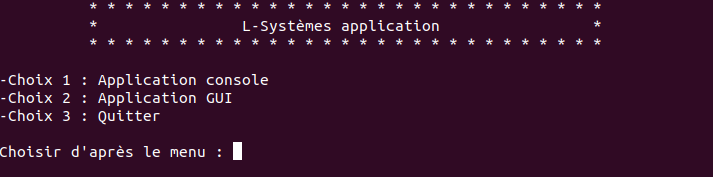
\includegraphics[width=12cm]{images/cap.png}
      \end{center}
        \caption{Mode Console}
        \label{fig:paquetage}
    \end{figure}
    
     \Large{Après vous pouver continuer avec vos choix saisis}
     \begin{itemize}
         \item (choix \textbf{2})
          \begin{figure}[h]
      \begin{center}
         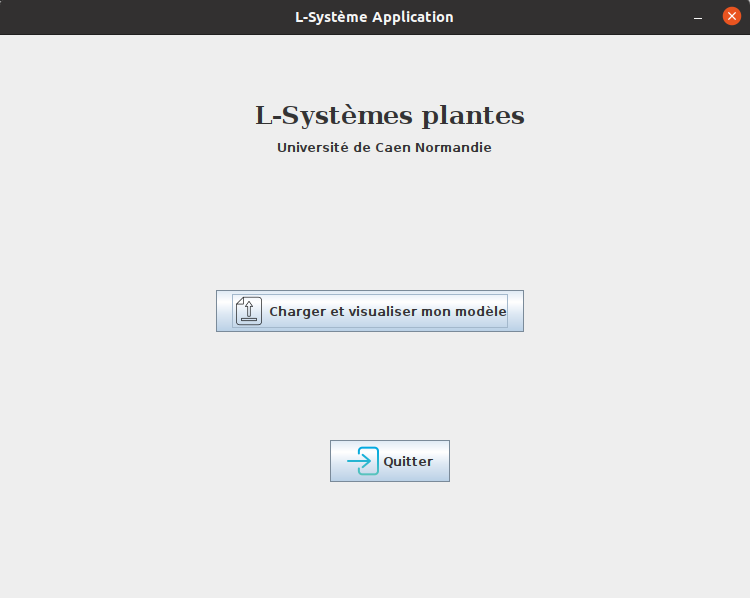
\includegraphics[width=9cm]{images/cap2.png}
      \end{center}
        \caption{Mode Graphique}
        \label{fig:paquetage}
    \end{figure}
     \end{itemize}
        
        
    \end{onehalfspace}
    \newpage
    \subsection{Résultats}
    \Large{"Comme vous allez voir le résultat du compilation ci-dessus. 
    Maintenant on pourra visualiser notre plante"}
      \begin{figure}[h]
      \begin{center}
         
\includegraphics[width=9cm]{images/arbre.png}
      \end{center}
        \caption{Résultat d'interprétation}
        \label{fig:paquetage}
    \end{figure}
    
   \Large{Et de plus on pourra enregistrer l'image déssinée}
    
    \begin{figure}[!h]
      \begin{center}
         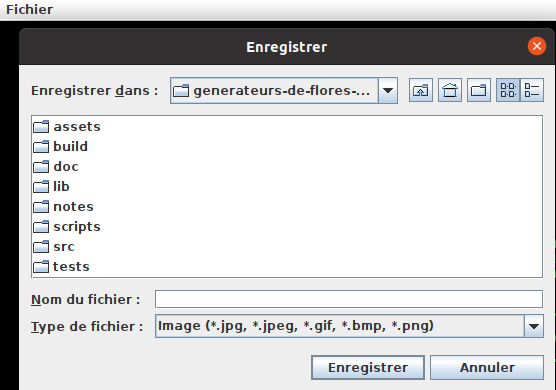
\includegraphics[width=9cm]{images/save.png}
      \end{center}
        \caption{Possibilité de sauvegarder l'image}
        \label{fig:paquetage}
    \end{figure}
    
    \subsection{Paquetage et structure du projet}
    \begin{figure}[h]
      \begin{center}
         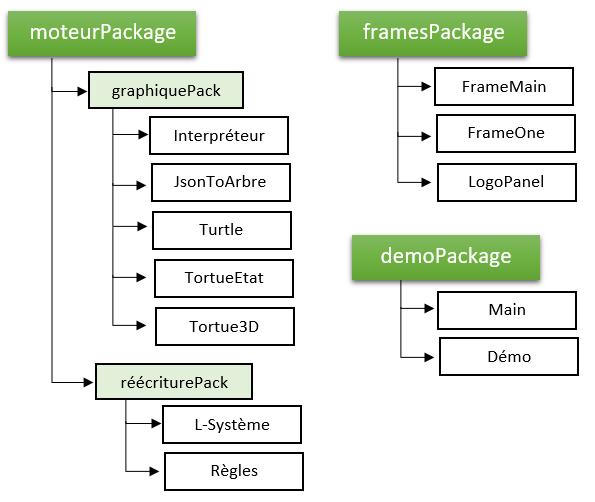
\includegraphics[width=12cm]{images/paquetage.png}
      \end{center}
        \caption{Paquetage du projet }
        \label{fig:paquetage}
    \end{figure}
    \vspace{1cm}
    \begin{onehalfspace}
    \Large{\texttt{moteurPackage} : gestion du système de réécriture du rendu graphique.}
    
     \Large{\texttt{framesPackage} : Ce package gère les interfaces graphqiues.}
     
    \Large{\texttt{demoPackage} : Le package de démonstration. }
    \end{onehalfspace}
    
    
    \newpage

     \newpage
    
\section{Architecture du projet}
    \subsection{Modélisation UML}
    
    \begin{figure}[h]
      \begin{center}
         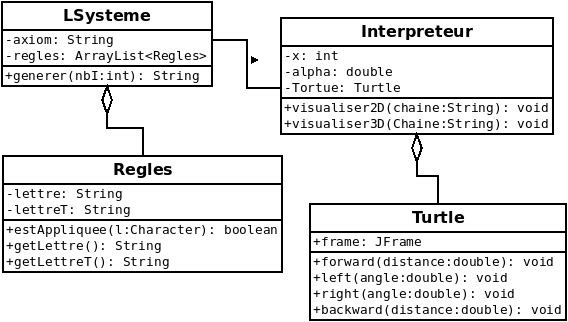
\includegraphics[scale=\umlscale]{diagrammes/interpretation.png}
      \end{center}
      \caption{Diagramme de gestion interpratation }
      \label{fig:interprete}
    \end{figure}
    
     \begin{figure}[h]
      \begin{center}
         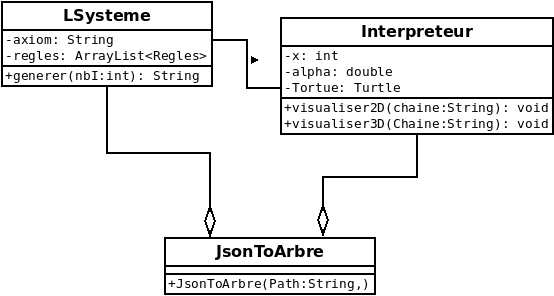
\includegraphics[scale=\umlscale]{diagrammes/json.png}
      \end{center}
        \caption{Diagramme de gestion de visualisation d'après un fichier JSON }
        \label{fig:json}
    \end{figure}
    
     \begin{figure}[!h]
      \begin{center}
         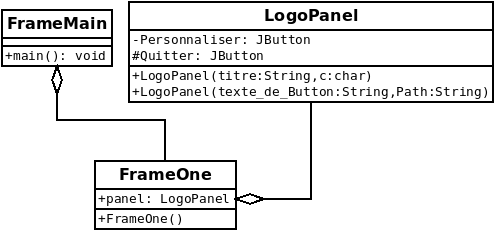
\includegraphics[scale=\umlscale]{diagrammes/graphique.png}
      \end{center}
        \caption{Diagramme de gestion des interfaces graphique }
         \label{fig:graphique}
    \end{figure}
    
   
      \begin{center}
         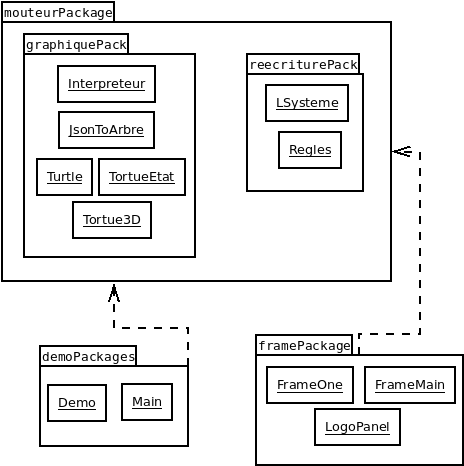
\includegraphics[scale=\umlscale]{diagrammes/paquetage.png}
      \end{center}
      \begin{center}
          \large{\textsc{Figure 6 - }Diagramme de paquetage}
      \end{center}
        
        
   
  


\newpage
    \subsection{Cas d’utilisation}
    \begin{onehalfspace}
          \Large{On a pris l'exemple de visualiser2D, il va falloir en avance une chaîne de caractères générés par la méthode Générer ainsi que cette méthode marche si chaque règle est appliquée, et pour elle fait appel à la méthode esAppliquée}  
    \end{onehalfspace}

    
    \begin{figure}[!h]
      \begin{center}
         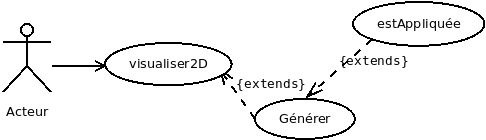
\includegraphics[scale=\umlscale]{diagrammes/usecase.png}
      \end{center}
        \caption{Cas d'utilisation de l'action "visualiser2D" }
        \label{fig:usecase}
    \end{figure}
    
\section{conclusion}
    \subsection{Récapitulatif des fonctionnalitées principales}
    \begin{onehalfspace}
    \Large{Le projet L-Système était une occasion pour maitriser beaucoup de notions
    en langage Java ainsi d'implémenter plusieurs fonctionnalitées, on cite :}
    
    \vspace{0.5cm}
    \Large{\texttt{Réaliser un système de réécriture} : pour qu'on puisse
    avoir une chaîne de caractères rédigée sous des règles et selon un nombre
    d'itérations.}
    
    \vspace{0.5cm}
    \Large{\texttt{Réaliser un moteur de rendu graphique} : pour qu'on puisse
    visualiser un arbre. Chaque caractère de la chaîne correspond à une interprétation graphique. Visualisation en 2D ou 3D.}
    
    \vspace{0.5cm}
    \Large{\texttt{Réaliser une interface graphique} : L'interface graphique cible aux utilisateurs qui ne préférent pas travailler sous commandes en mode console. En effet, on a créé une interface graphique avec laquelle l'utilisateur va intéragir.}
    
    \vspace{0.5cm}
      \Large{\texttt{Manipuler les fichiers JSON} : Il permet de représenter de l’information structurée. Dans notre cas, on a besoin de stocker des règles:}
      \begin{itemize}
          \item Axiom 
          \item Angle
          \item Nombre d'itérations
      \end{itemize}
    \end{onehalfspace}

    \subsection{Proposition d'améliorations}
    \begin{onehalfspace}
        \Large{Dans le cade de perfectionnement, le projet a plusieurs propositions d'améliorations. Voici une liste :}
         \vspace{0.5cm}
      \begin{itemize}
          \item \texttt{Extension ".lsy"} : \Large{Sachant que l'evolution de l'utilisation des L-Systèmes, pourquoi pas on crée une extension ".lsy" qui est une format d'un fichier qui stocke tous les données d'un modèle.}
        \vspace{0.5cm}
          \item \texttt{Jeu video} : \Large{À l'aide d'un "Game Engine" comme LWJGL\footnote{Lightweight Java Game Library est une bibliothèque de logiciels open source qui fournit des liaisons à une variété de bibliothèques C pour les développeurs de jeux vidéo vers Java.}, on peut décorer un jeu avec nos propres plantes créées avec L-Systèmes. }
       
      \end{itemize}
       
        
        \Large{}
        \Large{}
    \end{onehalfspace}
    
    







